上述篮球的基础数据是观众了解一个球员,球队的最直观方法也是观看比赛后评估一个球员表现的最直观的方法,但是Mark Cuban认为在专业篮球运动员分析某球队和某球员的具体表现和如何提高球队比赛效率,提高球员有效得分率,提高球员价值上仅仅利用简单的基础数据是远远不够的。这时需要利用数据来建立高级篮球分析指标,而这些指标可能对观众来说是没有实际意义的。本文将提取教练或篮球分析员最关注的指标:本文的指标构建分为两部分:第一部分是个体球员的指标构建,主要是在基础篮球数据的 基础上根据需求设计高级指标,在衡量运动员水平的时候包括衡量球员价值、球员效率、球员控球、球员实际命中率、球员有效得分率等;然后将个体球员数据整合到其球队的数据中,代表该球队整体球员的指标;第二部分考虑球队指标,球队指标包括球队排名、球队比分差距、球队的攻守效率,和作为我们预测结果的球队胜率:




\begin{enumerate}
	\item 个体球员指标:
	\begin{enumerate}
	
		
		
		
		
	
	
		\item True Shooting Percentage实际命中率:实际命中率等于个体球员在场上的总得分,除以运动员在赛场上所有投篮次数和罚球次数应得的分数 \\
		相对于衡量一个球员所有的投篮命中率,实际命中率更全面涵盖一个球员通过投篮得到所有的分数,包括二分球,三分球和罚球得分,该指标可以很客观的评判运动员的命中率高低,从而衡量一个球员的命中率对球队的贡献。\\
		
		\begin{align}
			True shooting Rate =  \frac{Points}{2*(Field Goal Attempt + 0.44*Free Throw Attempt)}
		\end{align}
		注释:系数0.44是根据一个球员每100次控球中2分球和3分球的出手比例计算而来的。如果100次控球中所有的投篮都是2分球,该系数应该是0.5,如果100次控球中所有投篮出手都是3分球,该系数为0.333.
	
		\item Effective Field Goal Percentage有效得分率:得分效率是每个球员在场上除了罚球命中之外的投球命中除以总投球次数,这里假设除了投球以外的命中得分均分为2分,所以利用总得分减去罚球得分除以2来近似所有除去罚球之后的投球命中次数。\\由于衡量命中率之后需要考虑每次命中的实际得分,由于3分球出手命中后得3分,2分球出手后命中得2分,不能用统一的标准来计算所有命中的得分。计算有效得分率,可以更好的衡量球员得分对整体球队的贡献。
		
		\begin{align}
		eFG Rate = \frac{(Points-FT)/2}{FGA}
		\end{align}
	
		\item PER:\cite{hollinger2005pro}衡量球员效率的指标Per Efficiency Rating. 指标根据NBA官网公开的各球员、球队、联盟的基础数据计算得出。总结球员对球队的正向贡献和负向贡献,即在衡量球员得分的指标前赋予一个正的系数,在衡量球员失分的指标前赋予一个负的系数,再将所有加权后的指标相加,再除以根据球队和联盟数据构建的指标对球员的数据进行规范化。PER最终得到球员每分钟的贡献率,该指标不应该受到球员上场时间,球队进攻类型,整个联盟赛制变化的影响。该指标客观有效的衡量球员的比赛效率,可以成为衡量球员对球队贡献指标之一。\\ 首先定义三个参数:
		\begin{align}
			Factor &= \frac{2}{3} - \frac{(0.5 * (League Assists / League Field Goal))}{(2 * (League Field Goal / League Free Throw))}\\
			DRB\%   &=  \frac{(League Total Rebounds - League Offensive Rebound)}{League Total Rebounds}
		\end{align}
		
		\begin{multline}
			VOP   =  League Points / (League Field Goal Attempt - League Offensive Rebound \\+ League Turnovers + 0.44 * League FreeThrowAttempts)
		\end{multline}
 依据上述三个参数,我们定义PER指标的计算公式
 \begin{multline}
 uPER = (1 / Minue Play) *
 [ 3Point
 + (2/3) * Assists
 \\+ (2 - Factor  * (Team Assists / Team Field Goal)) * Field Goal
 \\+ (Free Throw *0.5 * (1 + (1 - (Team Assists / Team Field Goal)) \\+ (2/3) * (Team Assists / Team Field Goal)))
 \\- VOP * Turnovers
 - VOP * DRB\%* (Field Goal Attempt - Field Goal)
 \\- VOP * 0.44 * (0.44 + (0.56 * DRB)) * (Free Throw Attempt - Free Throw)
 \\+ VOP * (1 - DRB\%) * (TotalRebound - Offensive Rebound)
 \\+ VOP * DRB\% * Offensive Rebound
 + VOP * Steal
 + VOP * DRB\% * Block
 \\- Personal Fouls * ((League Free throw / League Personal Fouls) - \\0.44 * (League FreeThrowAttempt / LeaguePersonalFouls) * VOP) ]
 \end{multline}
	注释:由于在大多数开源的数据中更多记录了一个球员进攻表现(更容易记录)如进攻篮板球,三分球得分,罚球得分等;记录球员防守表现的数据更少(不容易被记录)。所以该指标对一个防守很强的球员更有倾向。在实际应用中,两个同样优秀的球员,其一打球风格更激进,其二防守表现突出,可能PER在得出第一位球员更优秀的结论。	
	
	\item Usage percentage利用效率:在一场比赛中某队某球员掌控的控球机会比整个球队掌握的控球机会,在这里假设每个球队5个球员均等占据比赛时间;所以将整体球队的比赛时间除以5,代表每个球员的比赛时间,球员和球队的控球机会是投球次数和0.4倍的罚球次数和犯规次数的和。\\
	球员利用率是衡量每个球员在每一次掌握球权时对球权的利用率。根据射门次数、罚球次数、平局次数或失误次数等数据构建出该指标。通常控球次数多的球员有更高的利用效率,因此一般个子大的球员对球的控制能力更强,打出更高的利用效率。利用效率越高,相对球员效率PER越低。优秀的球员可以在最少的控球次数中打出最高的得分。
	
	\begin{multline}
		Usage percentage = 100 * ((FieldGoalAttempt + 0.44 * FreeThroaAttempt + Turnover) \\* (Team MinutePlay / 5)) / (MinutePlay * (Team FieldGoalAttemt \\+ 0.44 * Team FreeThrowAttempt + Team Turnover))
	\end{multline}
	
	
	
	\end{enumerate}
	
	
	



			
		\item 球队自身数据:
		
		\begin{enumerate}
		
		\item Team Rank:球队排名,依据球队赢得比赛的次数,与球队整个赛季中各个方面的表现得到的整体排名。排名综合考虑球队的进攻,防守,总得分和整体数据得出。
		\item Adjust MoV:调整后的Margin of Victory 比分差距是用来衡量比赛中获胜队伍和失败队伍比赛分数差距的统计量,参考MOV可以快速看出比赛是否激烈,获胜队伍胜利的是否显著,大的比分差距代表比赛中获胜方在比赛中强势压制对手,而小的比分差距说明两个球队水平接近,比赛相当激烈。在本数据集中,MOV指标是取一个队在整个赛季比赛中球队MOV指标的平均值。如果一个球队的Margin of Victory指标是正数,说明该球队在整个赛季中表现更好。然而在比赛中由于每个球队的进攻风格不同,需要按照进攻强度来调整对应的MOV值。尤其是不同的队伍会根据遇到的对手球队调整进攻步伐和阵容等,所以我们利用更好反映球队强弱的Adjust Mov数据来建模。历史上最大的比分差是68分,是1992年克利夫兰骑士队和迈阿密热火队的比赛,当时骑士队是最强的球队之一。
			\item
		Possession控球\cite{kubatko2007starting}:某个球队在控球表示该球队的队员在运球,传球,拿球;当防守球队控球,或者本球队队员投球(命中或否)代表本球队的控球结束。分析员在分析每场比赛数据时开始更加重视每次进攻数据或者每100次进攻的数据,根据基础得分数据可以得到每队在每场比赛中的得分,但是计算控球次数是很难的,因为某队的控球可以以4种方式结束:(1)该队球员投球命中;(2)该球队进攻犯规;(3)本球队投篮未命中;(4)球队队员进行外线投篮,投中2分或3分球,或者没有抢到篮板球,球权落到了对手中。虽然前三种很容易可以从基础数据中得到,但是第四种是很难得到的。\\
		一场比赛的控球次数等于一个球队的除去进攻篮板球的投球次数加犯规次数加0.436*罚球次数,因为根据以往数据得到结论某队43.6\%的罚球导致本队的控球结束。由于仅仅简单的将这些变量进行组合会导致严重高估每个球队的控球次数。本文将对计算方式进行调整。\\
		根据上述四种方式我们写出球队控球次数的计算公式,该公式分为两部分,第一部分是本球队的控球次数,第二部分是对手球队的控球次数,因为两个球队之间控球次数会因为进攻风格不同而导致两球队的控球次数有一定的差距,但在一场比赛中假设两个球队拥有相同的进攻次数,所以在这里取两个球队的控球次数和的平均。该公式仍然采取总投球次数加犯规次数加0.4的罚球次数,但是在这里将进攻篮板球进行加权后减去,权重等于该球队进攻篮板球与总篮板球的比例乘系数1.07,该系数根据往数据得到。然后用对手球队的数据重复上述运算,得到第二部分的数值。得到公式如下:
		
		\begin{multline}
		Possession = 0.5 * ((Team Field Goal Attepmt + 0.4 * Team Free Throw Attempts \\- 1.07 * (Team Offensive Rebounds / (Team Offensive Rebounds \\+ Opponent Defensive Rebounds)) * (Team Field Goal Attepmt \\- Team Field Goal) + Team Turnovers +(Opponent Field Goal Attepmt \\+ 0.4 * Opponent Free Throw Attempts- 1.07 * (Opponent Offensive Rebounds \\/ (Opponent Offensive Rebounds + Team Defensive Rebounds)) \\* (Opponent Field Goal Attepmt - Opponent Field Goal) + Opponent Turnovers))
		\end{multline}
		
	
		\item Winratio:在整个赛季的比赛中,赢得的比赛与参加的比赛之比作为胜率。胜率对衡量球队在下一个赛季的表现有着很重要的作用。可以帮助教练调整训练节奏和步伐,帮助球员在选秀中找到一个更合适自己的队伍,可以帮助粉丝们在赌球中有一个更好的判断。胜率的平均值在0.5.
				\begin{figure}[h]
			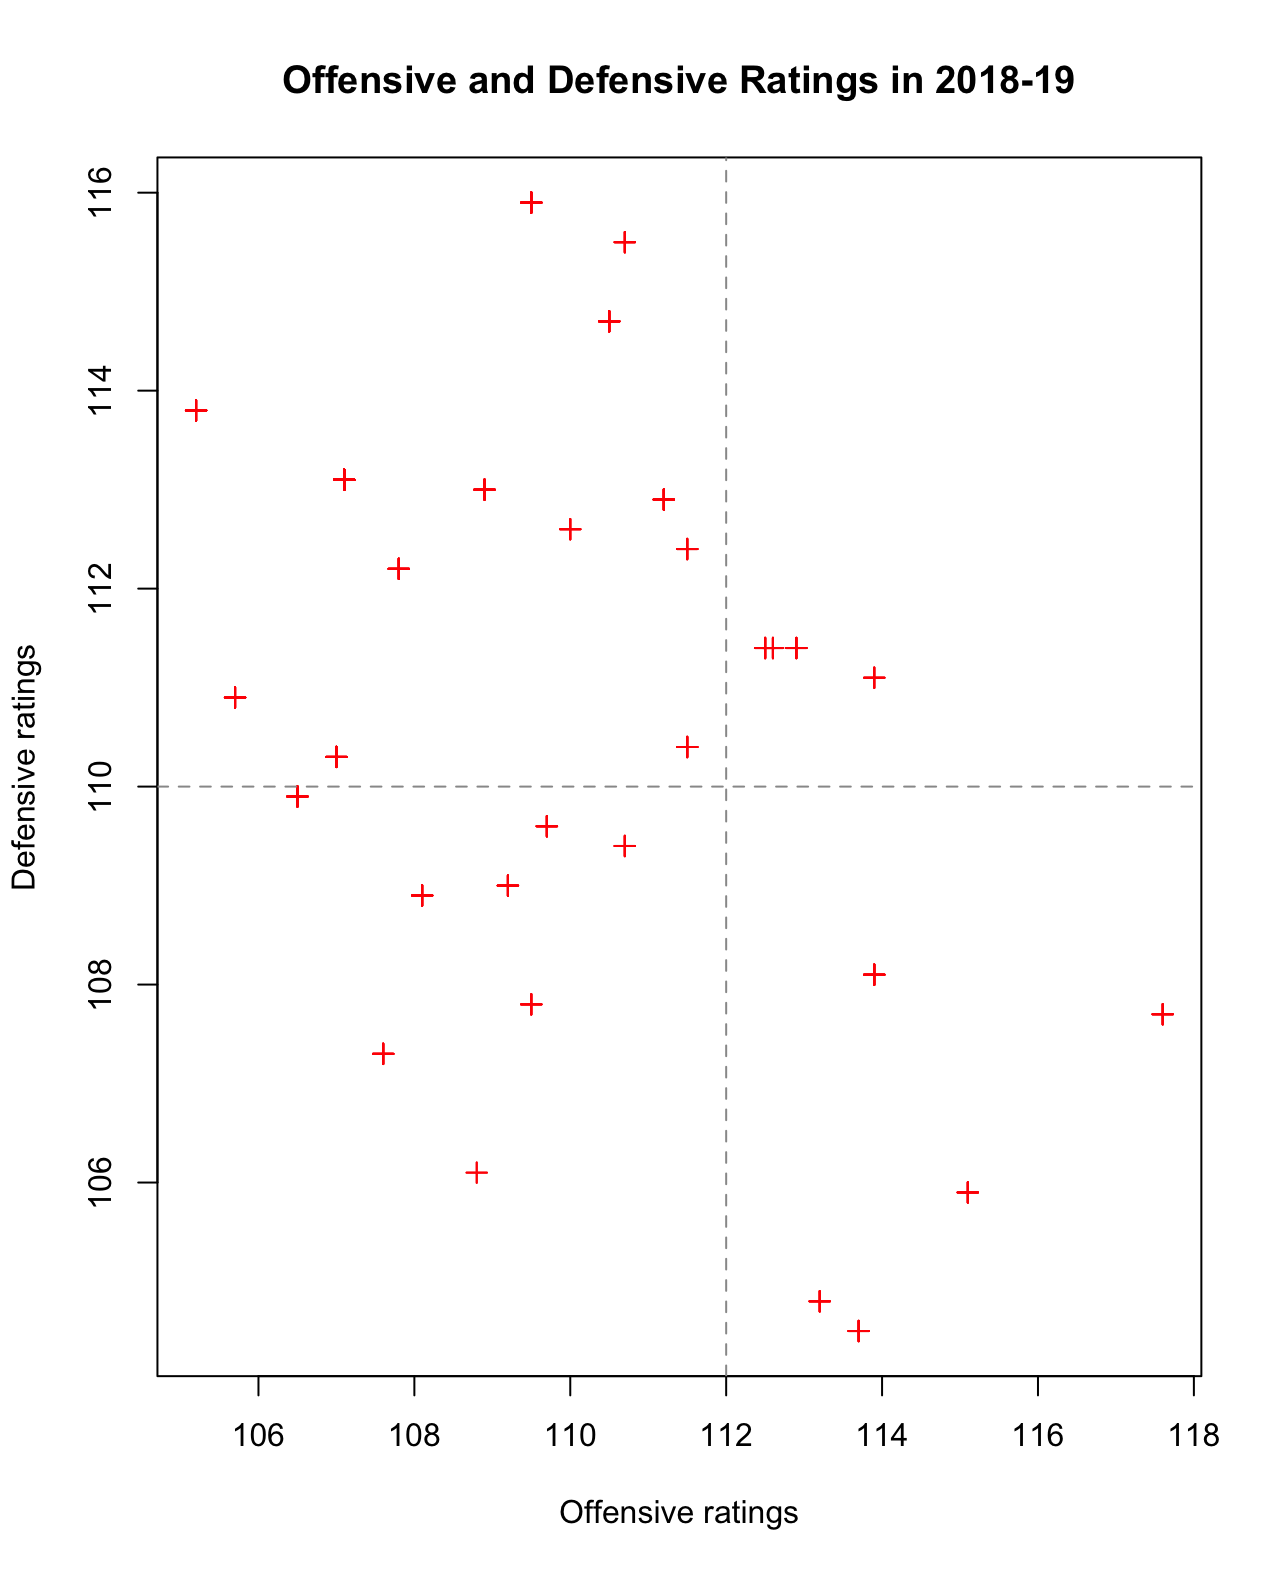
\includegraphics[width=10cm]{ORgtDRgt.png}\label{fig:1}
			\centering
			\caption{攻击效率和防守效率}
		\end{figure}
		\item Offensive and Defensive Ratings进攻得分和防守失分率: 率代表每次控球的得分(失分),进攻得分率和防守失分率是根据每100次控球的总得分或者对手球队得分。根据分别考虑进攻得分和防守失分可以全面的评判一个球队的能力和长处,而不是将目标只局限于得分高低。下图展示了2018-19赛季中顶级30个球队得分率和失分率的分布图。下边的球队防守能力更强,因为对方球队的得分较低;右边的球队进攻能力很强,因为进攻得分很高。 如果只单纯根据Offensive Rating和 Defensive Rating来衡量一个球队的优秀程度多少有一些偏差,这时需要引入球队净得分来更全面的衡量。Net Rating是球队每100次进攻中得分与失分的差。用来衡量球队风格,和更全面的评判球队的表现。一个球队如果在整个赛季中净得分大于0,说明进攻性更强。当然球队的净得分和球员的表现有很大的关系。球队的净得分均值是0. 
	
		\item Pace Adjustment 进攻效率调整:一个获得100次球权的 球队,比一个获得80次进攻机会的球队多25\%的机会进行投篮,助攻,篮板等,所以当两个球队有不同的控球次数时,需要调整获得的数据。不同的控球次数来源于球队不同的进攻风格,若一个球队的步伐相对缓慢,称为有更少的进攻机会。根据调整球队进攻步伐获得更统一的衡量标准。
		
		\end{enumerate}
		
	\end{enumerate}


\noindent 将个体球员指标转化为整个球队整体球员的指标:\\按照每支球队整个赛季中各个球员在场时间将球员排序,将个体球员构建四个指标分别和上场时间相乘,将每队上场时间最长的12个球员的上述指标与上场时间相乘后的指标相加得到某球队整体球员效率,整体球员命中率,整体球员有效利用率,和整体球员得分率。\\
该计算方法的意义:
	\begin{enumerate}
		\item  由于个体球员的指标与该赛季球员的比赛时长相关,该方法以时间作为权重,对球队球员的指标进行加权求和,返回整体球队球员的指标。
		\item 一些球员通过选秀等方式会被交易到其他球队,所以要计算球员上场时间最长的12个球员,更充分可以反映球员对球队的贡献。因为这12个球员是球队中比较稳定的中流砥柱.
		\item 该计算方法也可以自动给四个指标更高的球员赋予更大的权重,因为四个指标分别是衡量球员命中率,球员效率,球员利用率以及球员有效得分率的指标,指标值越高的球员上场时间可能更长,而指标值较低的球员的上场时间会相对较短,所以时长作为权重,可以很好的平衡球员之间的效率。
		
	\end{enumerate}
最终得到的指标分别为球队胜率W/L\%(因变量),比分差距MOV/A,球队攻击效率ORtg/A, 球队防守效率DRtg/A,球队净得分差NRtg/A, 球队实际命中率Team\_TSR, 球队球员有效得分率Team\_eFGP,球队有效利用率Team\_USR,球队整体球员效率Team\_PER,球队控球次数Team\_Poss。